\documentclass[10pt,t]{beamer}
\usepackage[utf8]{inputenc}
\usepackage[T1]{fontenc}
\usepackage{graphicx}
\usepackage{grffile}
\usepackage{longtable}
\usepackage{wrapfig}
\usepackage{rotating}
\usepackage{amsmath}
\usepackage{textcomp}
\usepackage{amssymb}
\usepackage{capt-of}
\usepackage{hyperref}
\usetheme{default}

% ---------------------------------------------------------------------

\author{L. Larrabee Strow}
\date{\today}
\title{\large The AIRS/CrIS/IASI (and CHIRP) \newline
 Radiatie Transfer Algorithms }
\subtitle{\footnotesize{AIRS Science Team Meeting}}
\date{\vspace{0.1in}\footnotesize{September 25, 2019 \vfill}}
\author{C. L. Hepplewhite\inst{1,2}, Sergio DeSouza--Machado\inst{1,2}, L. Larrabee Strow\inst{1,2}}
\institute[UMBC]{\inst{1} UMBC Physics Dept. \and \inst{2}UMBC JCET}
\input beamer_setup
\usetheme{metropolis}
\metroset{titleformat title=allcaps}
\renewcommand{\UrlFont}{\small\tt}
\renewcommand*{\UrlFont}{\footnotesize}
\tolerance=1000
\RequirePackage{fancyvrb}
\DefineVerbatimEnvironment{verbatim}{Verbatim}{fontsize=\footnotesize}
\begin{document}

\maketitle
\addtobeamertemplate{block begin}{
  \setlength{\parsep}{0pt}
  \setlength{\topsep}{3pt plus 2pt minus 2.5pt}
  \setlength{\itemsep}{0pt plus 0pt minus 2pt}
  \setlength{\partopsep}{2pt}
}

% --------------------------------------------------------------------
%%\section{Overview}
%\begin{frame}
%  \frametitle{Overview of talk}
%  \begin{itemize}
%  \item Current status.
%  \item Methods.
%  \item Programmatics.
%  \item Validation and sample results.
%  \item Plans.
    
%  \end{itemize}
%\end{frame}

% ---------------------------------------------------------------------
%%\section{Status}
\begin{frame}
  \frametitle{Status - 1}
  \begin{itemize}
  \item kCARTA calculations of layer-to-space optical depths for all parameters for the 49 and 703 SAF regression profiles for AIRS\_L1C, CrIS FSR and IASI are complete. 
  \item AIRS\_L1C and IASI SARTA update was released May and June this year.
  \item Updated version of AIRS using L1C channel set with SRFs referenced to 10-Sep-2010 drift corrected. 
  \item Spectroscopy based on HITRAN 2016 \& LBLRTM12.8 CO2,CH4 line mixing.
  \item The kCARTA ias used to generate TOA radiances to compare directly with SARTA for validation.
  \item CrIS FSR SARTA update for 2019 currently in work.
  
  \end{itemize}
\end{frame}

% ---------------------------------------------------------------------
\begin{frame}
  \frametitle{Status - 2}
  \begin{itemize}
  \item The 2019 SARTAs include the fixed gases, and variable O3, H2O, CO2, CH4, HNO3, N2O, SO2, NH3, the nonLTE and improved reflected surface thermal. 
  \item The new SARTA includes hooks to HDO algorithm, the computation is turned off.
  \item HDO regression is in progress, regression residuals up to 10\% rms. DIfferent method required for MW than for SW bands. Method based on depletion relative to standard abundance.
  \item To start on SARTA for CHIRP in due course.
    
  \end{itemize}
\end{frame}

% ---------------------------------------------------------------------
%\section{Methods}
%\begin{frame}
%  \frametitle{}
%  \begin{itemize}
%  \item 
%  \item 
%  \item 
%  \item 
%  \item 
    
%  \end{itemize}
%\end{frame}

% ---------------------------------------------------------------------
%\section{Programmatics}
%\begin{frame}
%  \frametitle{}
%  \begin{itemize}
%  \item 
%  \item 
%  \item 
%  \item 
%  \item 
    
%  \end{itemize}
%\end{frame}

% ---------------------------------------------------------------------
%\section{Results}
%\begin{frame}
%  \frametitle{}
%  \begin{itemize}
%  \item 
%  \item 
%  \item 
%  \item 
%  \item 
    
%  \end{itemize}
%\end{frame}

% ---------------------------------------------------------------------
\begin{frame}
  \frametitle{Results - IASI}
  \begin{center}
    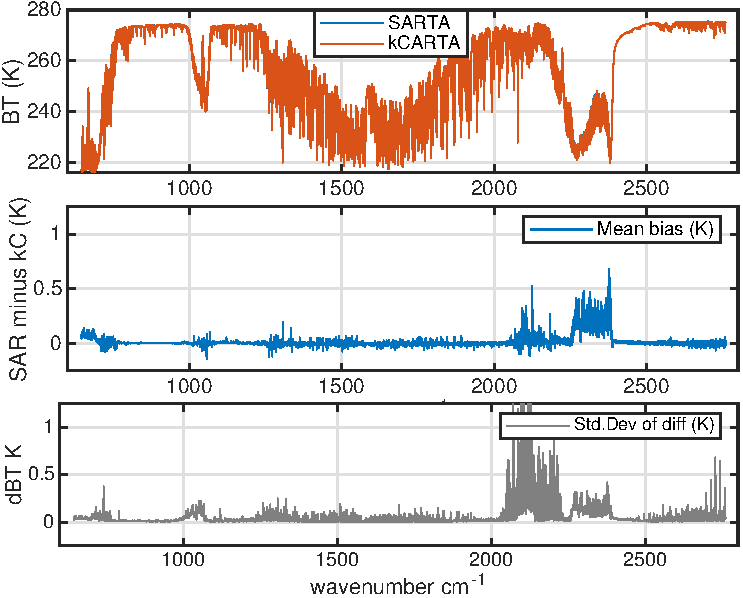
\includegraphics[width=0.9\linewidth]{./Figs/Pdf/kc_sar_iasi_mean_bias_stdv_sea_6angs_aslp.pdf}
  \end{center}
      
 \end{frame}

% ---------------------------------------------------------------------
\begin{frame}
  \frametitle{Results - AIRS\_L1C}
  \begin{center}
    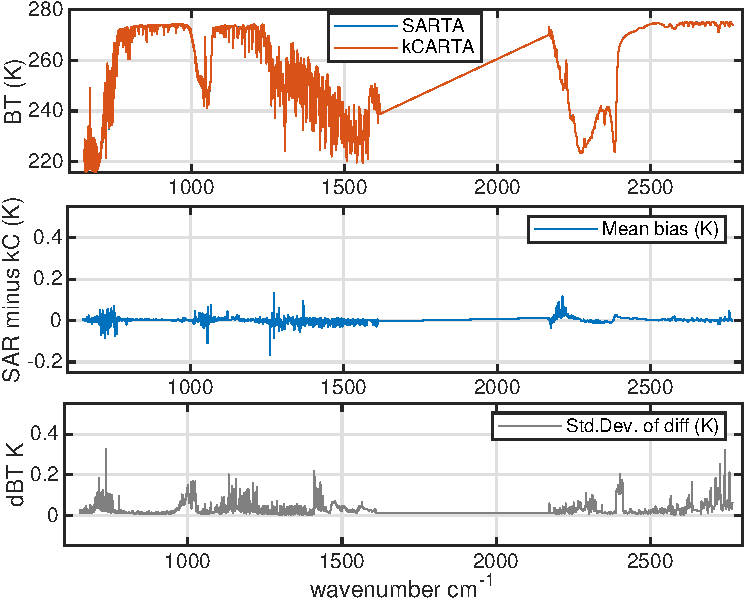
\includegraphics[width=0.9\linewidth]{./Figs/Pdf/kc_sar_airs_l1c_mean_bias_stdv_sea_6angs_aslp.pdf}
  \end{center}
      
 \end{frame}

% ---------------------------------------------------------------------
\begin{frame}
  \frametitle{Results - AIRS\_L1C Mean \& Std. Dev vs angle}

  \begin{center}
    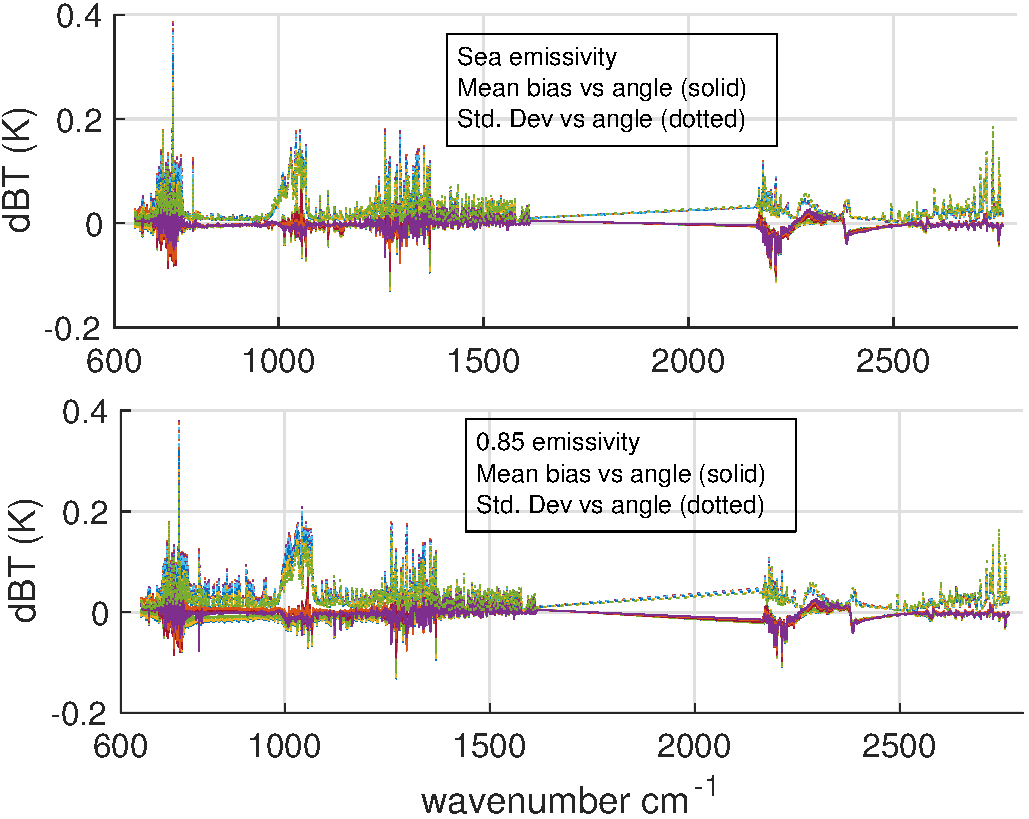
\includegraphics[width=0.9\linewidth]{./Figs/Pdf/kc_sar_airs_l1c_mean_stdv_emiss_vs_angle_v2.pdf}
  \end{center}
  
  \end{frame}

% ---------------------------------------------------------------------
%\section{Plans}
%\begin{frame}
%  \frametitle{Current and future Plans}
%  \begin{itemize}
%  \item 
%  \item 
%  \item 
%  \item 
%  \item 
    
%  \end{itemize}
%\end{frame}

% ---------------------------------------------------------------------

\end{document}
